\documentclass{article}
\usepackage[english]{babel}
\usepackage[a4paper,top=2.54cm,bottom=2.54cm,left=2.54cm,right=2.54cm,marginparwidth=1.75cm]{geometry}
\usepackage{amsmath}
\usepackage{graphicx}
\usepackage{amsfonts}
\usepackage{amssymb}
\usepackage{enumerate}
\usepackage{enumitem}
\usepackage[colorlinks=true, allcolors=blue]{hyperref}
\usepackage{graphicx}
\usepackage[export]{adjustbox}
\usepackage{multirow}
\usepackage{MnSymbol}%
\usepackage{wasysym}%
\title{Calculus A(1): Homework 7}
\begin{document}
\maketitle
\section*{3.7.}
\subsection*{24.}
\textbf{Making coffee} Coffee is draining from a conical filter into a cylindrical coffeepot at the rate of 10 in$^3$/min.
\begin{enumerate} [label=\textbf{\alph*.}]
    \item How fast is the level in the pot rising when the coffee in the cone is 5 in. deep?
    \item How fast is the level in the cone falling then?
\end{enumerate}
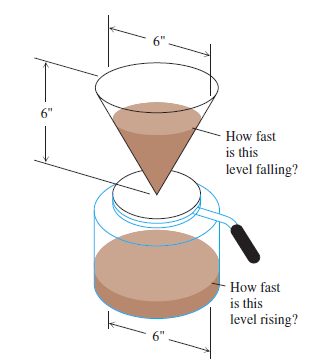
\includegraphics[]{img/20211129_calculusA_HW7_Fig_1.PNG}
\subsection*{Solution.}
Denote $V(t)$ as volume of coffee in the pot, $h_1(t)$ as the height of level in the pot measured from the bottom, $h_2(t)$ as the height of level int the cone measured from the bottom of the cone.
\begin{enumerate} [label=\textbf{\alph*.}]
    \item 
    Consider the pot.
    \[\frac{dV(t)}{dt}=\frac{9\pi h_1(t)}{dt}=9\pi \frac{dh_1(t)}{dt}=10\]
    Hence, the level is rising at $\frac{10}{9\pi}$ in/min when the coffee in the cone is 5 in deep.
    \item 
    Consider the cone.
    \[\frac{dV(t)}{dt}=\frac{d(\pi(h_2(t)/2)^2\cdot h_2(t)/3)}{dt}=\frac{\pi}{12}\frac{d(h_2(t)^3)}{dt}=\frac{\pi}{4}h_2(t)^2\frac{dh_2(t)}{dt}=-10\]
    \[\Rightarrow \left.\frac{dh_2(t)}{dt}\right\vert_{h_2(t)=5}=-\frac{40}{25\pi}=-\frac{8}{5\pi}\]
\end{enumerate}
\section*{3.8.}
\subsection*{61.}
\textbf{The linearization is the best linear approximation} (This is why we use the linearization.) Suppose that $y=f(x)$ is differentiable at $x=a$ and that $g(x)=m(x-a)+c$ is a linear function in which $m$ and $c$ are constants. If the error $E(x)=f(x)-g(x)$ were small enough near $x=a$, we might think of using $g$ as a linear approximation of $f$ instead of linearization $L(x)=f(a)+f'(a)(x-a)$. Show that if we impose on $g$ the conditions
\begin{enumerate}
    \item $E(a)=0$
    \item $\lim _{x\to a} \frac{E(x)}{x-a}=0$
\end{enumerate}
then $g(x)=f(a)+f'(a)(x-a)$. Thus, the linearization $L(x)$ gives the only linear approximation whose error is both zero at $x=a$ and negligible in comparsion with $x-a$.\newline
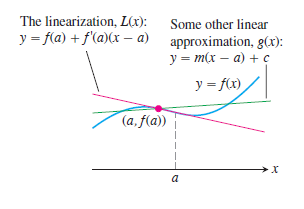
\includegraphics[]{img/20211129_calculusA_HW7_Fig_2.PNG}
\subsection*{Solution.}
The first condition implies that $f(a)=g(a)=m(a-a)+c=c$.\newline
The second condition can be rewritten as
\[\lim _{\Delta x\to 0} \frac{E(a+\Delta x)-E(a)}{\Delta x}=E'(a)=0\]
\[\Rightarrow f'(a)=g'(a)=m\]
Hence, enforcing the conditions immediately gives
\[g(x)=f(a)+f'(a)(x-a)=L(x)\approx f(x), x\to a \]
is in the small neighborhood of $a$.
\section*{4.1.}
\subsection*{54.}
Let $f(x)=\vert x^3-9x\vert$.
\begin{enumerate} [label=\textbf{\alph*.}]
    \item Does $f'(0)$ exist?
    \item Does $f'(3)$ exist?
    \item Does $f'(-3)$ exist?
    \item Determine all extrema of $f$.
\end{enumerate}
\subsection*{Solution.}
\[f(x)=\left\{\begin{array}{ll}
-x^3+9x, & x<-3\lor 0\leq x <3 \\
x^3-9x, & -3\leq x <0 \lor x\geq 3
\end{array}\right.\]
\begin{enumerate} [label=\textbf{\alph*.}]
    \item 
    \[\lim _{h\to 0^-} \frac{f(h)-f(0)}{h}=\lim _{h\to 0^-} \frac{h^3-9h}{h}=\lim _{h\to 0^-} (h^2-9)=-9\]
    \[\lim _{h\to 0^+} \frac{f(h)-f(0)}{h}=\lim _{h\to 0^+} \frac{-h^3+9h}{h}=\lim _{h\to 0^+} (-h^2+9)=9\]
    \[\lim _{h\to 0^-} \frac{f(h)-f(0)}{h}\neq \lim _{h\to 0^+} \frac{f(h)-f(0)}{h},\]
    so $f'(0)$ does not exist.
    \item 
    \[\lim _{h\to 0^-} \frac{f(3+h)-f(3)}{h}=\lim _{h\to 0^-} \frac{-(3+h)^3+9(3+h)}{h}=\lim _{h\to 0^-} \frac{-h^3-9h^2-18h}{h}=\lim _{h\to 0^-} (-h^2-9h-18)=-18\]
    \[\lim _{h\to 0^+} \frac{f(3+h)-f(3)}{h}=\lim _{h\to 0^+} \frac{h^3+9h^2+18h}{h}=\lim _{h\to 0^+} (h^2+9h+18)=18\]
    \[\lim _{h\to 0^-} \frac{f(3+h)-f(3)}{h}\neq \lim _{h\to 0^+} \frac{f(3+h)-f(3)}{h},\]
    so $f'(3)$ does not exist.
    \item 
    \[\lim _{h\to 0^-} \frac{f(-3+h)-f(-3)}{h}=\lim _{h\to 0^-} \frac{-(-3+h)^3+9(-3+h)}{h}=\lim _{h\to 0^-} \frac{-h^3+9h^2-18h}{h}=\lim _{h\to 0^-} (-h^2+9h-18)=-18\]
    \[\lim _{h\to 0^+} \frac{f(-3+h)-f(-3)}{h}=\lim _{h\to 0^+} \frac{h^3-9h^2+18h}{h}=\lim _{h\to 0^+} (h^2-9h+18)=18\]
    \[\lim _{h\to 0^-} \frac{f(-3+h)-f(-3)}{h}\neq \lim _{h\to 0^+} \frac{f(-3+h)-f(-3)}{h},\]
    so $f'(-3)$ does not exist.
    \item 
    \[f'(x)=\left\{\begin{array}{ll}
    -3x^2+9, & x<-3 \lor 0<x<3 \\
    3x^2-9, & -3<x<0 \lor x>3
    \end{array}\right.\]
    \[f''(x)=\left\{\begin{array}{ll}
    -6x, & x<-3 \lor 0<x<3 \\
    6x, & -3<x<0 \lor x>3
    \end{array}\right.\]
    On one hand,let $x_0\in\mathbb{R}$ satisfies $f'(x_0)=0\Rightarrow 3x_0^2-9=0 \Rightarrow x_0=\pm\sqrt{3}$.
    \[f''(-\sqrt{3})=6(-\sqrt{3})<0,f''(\sqrt{3})=-6(\sqrt{3})<0\]
    Hence, $f$ has two extrema, both of which are maxima. The maxima are $x=\sqrt{3}$ and $x=-\sqrt{3}$.\newline
    On the other hand, $f(x)\geq 0$, and equality holds iff $x=-3\lor x=0\lor x=3$.\newline
    In conclusion, $f(-3)=0$, $f(0)=0$, $f(3)=0$ are global minima, and $f(-\sqrt{3})=6\sqrt{3}$, $f(\sqrt{3})=6\sqrt{3}$ are local maxima.
    
\end{enumerate}
\subsection*{61.}
\textbf{Area of a right triangle} What is the largest possible area for a right triangle whose hypotenuse is 5 cm long?
\subsection*{Solution.}
Let $a,b>0$ be the two other sides of the triangle.
So, it is a problem of maximizing $ab/2$ given $a^2+b^2=25$.\newline
By arithmetic-mean geometric-mean inequality, 
\[\text{Area of the triangle}=\frac{1}{2}ab\leq \frac{1}{4}(a^2+b^2)=\frac{25}{4}\]
\subsection*{70.}
\textbf{Functions with no extreme values at endpoints}
\begin{enumerate} [label=\textbf{\alph*.}]
    \item Graph the function 
    \[f(x)=\left\{\begin{array}{ll}
    \sin\frac{1}{x}, & x>0 \\
    0, & x=0.
    \end{array}\right.\]
    Explain why $f(0)=0$ is not a local extreme value of $f$.
    \item Construct a fucntion of your own that fails to have an extreme value at a domain endpoint.
\end{enumerate}
\subsection*{Solution.}
\begin{enumerate} [label=\textbf{\alph*.}]
    \item \textbf{ }\newline
    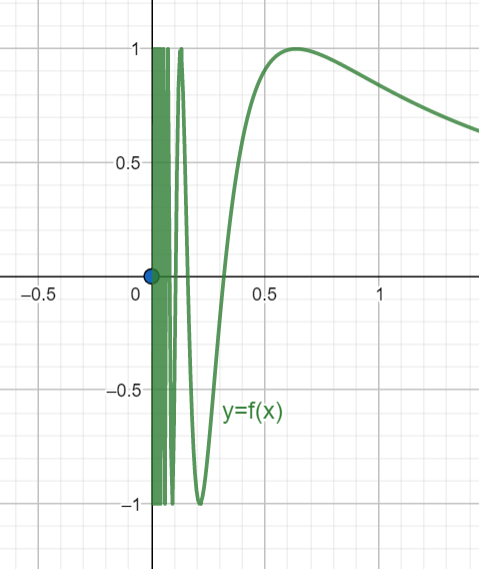
\includegraphics[scale=0.5]{img/20211202_calculusA_HW7_Fig_3.PNG}
    \newline
    A local extreme value $y_0=f(x_0)$ satisfies
    \[f(x)\leq y_0\]
    for all $x$ in some neighborhood of $x_0$, if it is a local maximum,
    and 
    \[f(x)\geq y_0\]
    for all $x$ in some neighborhood of $x_0$, if it is a local minimum.\newline
    As $f$ is defined on $[0,+\infty)$, we only discuss $x\in(0,\delta)$, $\delta>0$, that is all the points in the right $\delta$-neighborhood of 0.
    \[(\forall \delta>0)(\exists k\in \mathbb{Z}^+)(x_1=\frac{2}{(4k+1)\pi}\land x_2=\frac{2}{(4k-1)\pi}\land 0<x_1<x_2<\delta).\]
    However,
    \[f(x_1)=1,f(x_2)=-1\]
    Hence, there exists $x_1,x_2$ in any right neighborhood of 0, that $f(x_1)=-1<f(0)=0<f(x_2)=1$, and $f(0)=0$ is not a local extreme value.
    \item Let $g:[0,+\infty)\to [-1,1]$.
    \[g(x)=\left\{\begin{array}{ll}
    \sin\frac{2}{x}, & x>0 \\
    \frac{1}{3}, & x=0.
    \end{array}\right.\]
    Again, $g(0)=\frac{1}{3}$ is not a local extreme value of $g$, The proof is similar to (a), by switching all $f$ to $g$, and by letting $x_1=\frac{1}{(4x+1)\pi},x_2=\frac{1}{(4k-1)\pi}$ 
\end{enumerate}
\section*{4.2.}
\subsection*{10.}
For what values of $a,m$ and $b$ does the function 
\[f(x)=\left\{\begin{array}{ll}
3, & x=0 \\
-x^2+3x+a, & 0<x<1 \\
mx+b, & 1\leq x\leq 2
\end{array}\right.\]
satisfy the hypotheses of the Mean Value Theorem on the interval $[0,2]$?
\subsection*{Solution.}
$f$ is continuous on $[0,2]$. Thus,
\[\lim_{x\to 0^+}f(x)=\lim_{x\to 0^+} (-x^2+3x+a)=f(0)=3\Rightarrow a=3\]
\[\lim_{x\to 1^-}f(x)=\lim_{x\to 1^-}(-x^2+3x+3)=5=\lim _{x\to 1^+} f(x)=\lim _{x\to 1^+} (mx+b) =m+b\]
$f$ is differentiable on $(0,2)$. Thus,
\[\lim _{h\to 0^-}\frac{f(1+h)-f(1)}{h}=\lim _{h\to 0^+}\frac{f(1+h)-f(1)}{h}\]
\[\lim _{h\to 0^-}\frac{f(1+h)-f(1)}{h}=-2+3=1,\]
\[\lim _{h\to 0^+} \frac{f(1+h)-f(1)}{h}=m\]

Thus, $m=1,b=5-m=4$. In conclusion,
\[a=3,b=4,m=1\]
\subsection*{14.}
Show that a cubic polynomial can have at most three zeros.
\subsection*{Solution.}
Let $P(x)=ax^3+bx^2+cx+d,a\neq 0$. By definition, deg $P=3$, thus $P(x)$ is a cubic polynomial.
\[P'(x)=3ax^2+2bx+c\]
\[P''(x)=6ax+2b\]
\[P'''(x)=6a\]
Hence $P'''(x)$ is a non-zero constant.
Assume $x_1,x_2,x_3,x_4\in \mathbb{R}$ are all distinct that statisfies $P(x_1)=P(x_2)=P(x_3)=P(x_4)=0$.\newline
By applying Rolle's theorem for several times,
\[(\exists x_{11}\in(x_1,x_2))(\exists x_{12}\in(x_2,x_3))(\exists x_{13}\in(x_3,x_4))(P'(x_{11})=P'(x_{12})=P'(x_{13})=0)\]
\[\Rightarrow(\exists x_{21}\in(x_{11},x_{12}))(\exists x_{22}\in(x_{12},x_{23}))(P''(x_{21})=P''(x_{22})=0)\]
\[\Rightarrow(\exists x_{31}\in(x_{21},x_{22}))(P'''(x_{31})=0)\]
However, the last proposition is a contradiction to the fact that the third derivative of $P$ is a non-zero constant, hence a cubic polynomial cannot have more than 3 roots.
\subsection*{A1.}
Let $a<b$ and $f:[a,b]\to\mathbb{R}$ such that the derivative $f'$ of $f$ exists, $f'$ is continuous on $[a,b]$ and $f'$ is differentiable on $(a,b)$, and $f(a)=f(b)=0$. In particular, the second derivative $f''$ exists on $(a,b)$. Show that for any $x\in(a,b)$, there exists $c\in(a,b)$ such that 
\[f(x)=\frac{f''(c)}{2}\cdot (x-a)(x-b)\]
\subsection*{Solution.}
Define $g:[a,b]\to\mathbb{R}$ such that 
\[g:x\mapsto A(x-a)(x-b),\]
where $g$ has $g''$ exists on $(a,b)$, and $g'$ is continuous on $[a,b]$. $A\in\mathbb{R}$ is a constant to be determined from the behavior of $f$.\newline
Then, $\forall y\in (a,b)$,  $A$ can be chosen that satisfies 
\[f(y)=g(y)\]
\[\Rightarrow A=\frac{f(y)}{(y-a)(y-b)}\]
Define $h:[a,b]\to \mathbb{R}$ such that
\[h(x)=f(x)-g(x)\]
Clearly, $h''$ exists on $(a,b)$, and $h'$ is continuous on $[a,b]$. With the given conditions,
\[h(a)=h(y)=h(b)=0\]
Hence, as a consequence of Rolle's theorem, $\exists c_1\in (a,y), c_2\in (y,b)$ such that
\[h'(c_1)=h'(c_2)=0\]
\[\Rightarrow (\exists c\in(c_1,c_2))h''(c)=0\]
\[\Rightarrow f''(c)=g''(c)=2A=\frac{2f(y)}{(y-a)(y-b)}\]
\[\Rightarrow f(y)=\frac{1}{2}f''(c)(y-a)(y-b)\text{    }\blacksquare\]
\subsection*{B1.}
Let $f:[1,+\infty)\to \mathbb{R}$ be continuous on $[1,+\infty)$ and differentiable on $(1,+\infty)$. Determine if the following statements are true or false. If true, provide a proof and if false, give a counter-example.
\begin{enumerate}
    \item If $\lim_{x\to +\infty} f(x)=0$ and $\lim _{x\to +\infty} f'(x)$ exists, then $\lim_{x\to +\infty} f'(x)=0$.(Hint: apply the MVT on each segment $[n,n+1]$ for $n\in\mathbb{N}^*$.)
    \item If $\lim_{x\to +\infty} f(x)=0$, then $\lim _{x\to +\infty} f'(x)=0$.
\end{enumerate}
\subsection*{Solution.}
\begin{enumerate}
    \item True.\newline 
    $f$ is continuous on $[1,+\infty)$ and differentiable on $(1,+\infty)$, hence $\forall t\in \mathbb{N}^*$, $\exists c_t\in (t,t+1)$ such that 
    \[f'(c_t)=\frac{f(t+1)-f(t)}{t+1-t}=f(t+1)-f(t)\Leftrightarrow f(t+1)=f'(c_t)+f(t)\]
    Now we restrict $t$ such that for any given $M\in \mathbb{R}$, $t\geq M$. Then, by the existence of 
    \[\lim _{x\to +\infty} f'(t),\]
    \[\lim_{t\to+\infty}f(t+1)=\lim_{t\to +\infty}f'(c_t)+\lim _{t\to+\infty} f(t)\Rightarrow \lim _{t\to+\infty} f'(c_t)=0\]
    Therefore, \[f'(c_t),f'(c_{t+1}),f'(c_{t+2}),\cdots \to 0 \text{ when } t\to +\infty\]
    The existence of this sequence implies 
    \[\lim_{x\to+\infty} f'(x)=0 \text{    }\blacksquare\]
    \item False. \newline
    Consider $f(x)=e^{-x}\cos(e^x)$.\newline
    By definition, $f\in C^1$. Moreover,
    \[0=\lim _{x\to+\infty} -e^{-x}\leq \lim _{x\to+\infty} f(x) \leq \lim_{x\to+\infty} e^{-x}=0 \Rightarrow \lim _{x\to+\infty} f(x)=0\]
    Its derivative is
    \[f'(x)=-e^{-x}\cos(e^x)-e^{-x}\sin(e^x)\cdot e^x=-e^{-x}\cos(e^x)-\sin(e^x)\]
    Thus if the limit exists, then 
    \[(\exists A)(\forall \epsilon>0)(\exists M)(\forall x)(x>M\rightarrow |f'(x)-A|<\epsilon.\]
    Below chooses $k\in\mathbb{N}^*$ such that $k$ satisfies 
    $x=\ln{\frac{(4k-1)\pi}{2}}>M$. Clearly, $k$ exists.
    \[f'(x)=-\frac{2}{(4k-1)\pi}\cos\frac{(4k-1)\pi}{2}-\sin\frac{(4k-1)\pi}{2}=1\]
    Choose another $x$, for instance $x=\ln\frac{(4k+1)\pi}{2}$. Then,
    \[f'(x)=-\frac{2}{(4k+1)\pi}\cos\frac{(4k+1)\pi}{2}-\sin\frac{(4k+1)\pi}{2}=-1\]
    Hence, $A$ does not exist, which disproved the statement. $\blacksquare$
\end{enumerate}
\end{document} 